\documentclass[a4paper]{article}
\usepackage[margin=3cm]{geometry}
\usepackage[utf8]{inputenc}
\usepackage{cmbright}
\usepackage[hidelinks]{hyperref}
\usepackage{booktabs}
\usepackage[ngerman]{babel}
\usepackage{parskip}
\usepackage{graphicx}
\usepackage{minted}
\usepackage{pdflscape}
%\usepackage{array}
\usepackage{tabulary}
\usepackage{multicol}
\usepackage{pgfgantt}
\usepackage{pgf-umlcd}
%\usepackage{enumitem}
%\usepackage{pifont}
%\usepackage{threeparttable}

% Page breaks between sections
\let\oldsection\section
\renewcommand\section{\clearpage\oldsection}

% JIRA/Confluence shortcuts
\def\jiraurl{https://jira.keltec.ch/jira}
\def\confluenceurl{https://jira.keltec.ch/wiki}
\newcommand{\jiraissue}[1]{\href{\jiraurl/projects/EPJ/issues/EPJ-#1}{EPJ-#1}}
\newcommand{\fulljiraissue}[1]{EPJ-#1 (\url{\jiraurl/projects/EPJ/issues/EPJ-#1})}

% Tools
\newcommand{\tool}[2]{\emph{#1\footnote{\url{#2}}}}

\newcommand{\cmark}{\ding{51}}
\newcommand{\xmark}{\ding{55}}

\begin{document}
  \title{
    Projekt: kitovu \\
    \Large{Schlussbericht} \\[3em]
    
\includegraphics[width=20em]{../../img/logo/kitovu.jpg}
  }
  \author{
    Florian Bruhin \\ \url{florian.bruhin@hsr.ch} \and
    Méline Sieber \\ \url{meline.sieber@hsr.ch} \and
    Nicolas Ganz \\ \url{nicolas.ganz@hsr.ch}
    }
  \date{\today}

  \maketitle

  \section*{Änderungsgeschichte}

  \begin{tabulary}{\linewidth}{llLl}
    \toprule
    Datum & Version & Änderung & AutorIn \\
    \midrule
    16.05.2018 & 1.0 & Dokument erstellt und Struktur aus der Vorlage übernommen & Nicolas Ganz \\
    \bottomrule
  \end{tabulary}

  \pagebreak

  \section{Zielerreichung}

Dieses Projekt ist wohl eines der Ausnahmen in der Softwareentwicklung:

\begin{itemize}
  \item Wir haben alle gesetzten Ziele erreicht, sogar übertroffen, und das innerhalb der gesetzten Zeit.
  \item Die Kommunikation verlief reibungslos, sowohl online wie auch offline.
  \item Keine nennenswerten Konflikte innerhalb des Teams.
  \item Wir haben so gut wie immer die richtigen Entscheidungen gefällt, zu jedem Zeitpunkt des Projekts (Plugin-Architektur, Verteilung von Aufgaben, Grundsatzentscheidungen).
\end{itemize}

Als Hauptziel haben wir uns gesetzt, den Skripteserver anzubinden und eine erfolgreiche Synchronisation der benötigten Unterrichtsmaterialien durchzuführen. Das ist uns gelungen. Die beiden optionalen Erweiterungen, wie wir sie im Projektplan definiert haben, sind gleichzeitig die grösste Überraschung und grösste Enttäuschung:

Zu unserer grössten Überraschung haben wir es geschafft, Moodle in \emph{kitovu} einzubinden, was wir im Projektplan als grösstes Risiko identifiziert hatten. Unsere grösste Enttäuschung war hingegen, dass wir sehr bald das Studentenportal von unseren optionalen Anbindungen streichen mussten.

\section{Allgemeiner Erfahrungsbericht}

Wir haben \emph{kitovu} als kleines Projekt geplant, um einen möglichst hohen Lerneffekt zu erzielen: Für alle war es in der einen oder anderen Weise das erste, selber geführte Software-Projekt in einem kleinen Team. Es hat sich gelohnt, die Latte nicht zu hoch zu legen -- mit dem Resultat, dass wir alle Ziele erreicht haben und nun für die HSR ein nützliches Werkzeug bereitstellen können.

Folgende wichtige Entscheidungen haben auch dazu beigetragen:
\begin{description}
  \item[Erweiterbarkeit via Plugin-Architektur:] Erleichterte das Testen, aber auch die stückweise Erweiterung, zuerst mit dem Skripteserver, dann mit Moodle.
  \item[Code-Regeln setzen:] Wir setzten uns selber hohe Hürden, bis es Code in den Master-Branch schaffte: Pull-Requests, dann Code-Review eines Teammitglieds; gleichzeitig  Style-Prüfung mit Mypy, Flake8 und Pylint. Erst wenn der Code all diese Prüfungen passiert hatte, wurde er Teil des Masters.
  \item [Wöchentliche Meetings:] Sich jede Woche mindestens einmal zu dritt zu treffen hat sich ausbezahlt. Wir klärten viele Fragen, glichen unsere Projektvision an und konnten immer rechtzeitig den Verlauf anpassen.
  \item[Pair-Programming:] Sowohl erfahrene Programmierer wie Florian und Nicolas als auch Méline konnten viel voneinander lernen und profitieren.
  \item[Beschlüsse gemeinsam treffen:] Wichtige Designentscheide (FileCache, Error-Handling) haben wir gemeinsam im Team getroffen.
\end{description}

Alles in Allem nehmen wir alle drei sehr positive Erinnerungen von diesem Projekt mit, haben viel gelernt und werden nach Projektabschluss sicher noch daran weiterarbeiten. Und natürlich hoffen wir, dass viele HSR-Studentinnen und -Studenten \emph{kitovu} einsetzen werden.

  \section{Persönliche Erfahrungen}

  \subsection{Méline Sieber}

Nach diesem Engineering-Projekt weiss ich: Es gibt Einhörner.

Gruppenarbeitseinhörner. Solche Team-Arbeiten, in denen einfach alles rund und perfekt läuft. Ich staune noch jetzt, wie reibungslos alles lief. Als Quereinsteigerin war für mich so gut wie alles neu, so gut wie alles machte ich zum ersten Mal: Werkzeuge wie Jira, Github, Travis verwenden; ein Programm von Grund auf schreiben, also mehr als nur einen fehlenden Programmausschnitt ergänzen; im Team Software entwickeln.

Der Einstieg war erwartungsgemäss steil, das Wasser kalt. Viele Konzepte aus der Elaborationsphase verstand ich erst in der Anwendung (Travis, AppVeyor). Erst nach etwa zwei Sprints erhielt ich langsam ein Gefühl für die Arbeitsabläufe (Pull Requests, Code Reviews etc.). Glück im Unglück war der FileCache: Aufgrund krankheitsbedingter Abwesenheit von Florian fiel mir dieser anspruchsvolle Teil von kitovu zu. Dank dieser Aufgabe erreichte ich endlich die benötigte Programmierroutine. Das zu Beginn mir selber gesetzte Ziel habe ich erreicht, mehr Routine zu erlangen und flüssiger programmieren zu können. Des Weiteren wurde mir klar, wie wichtig Tests sind -- denn anhand dieser verstand ich nebenbei, wie Code funktioniert, den ich nicht selber geschrieben habe.

Ein unverzichtbarer, äusserst wertvoller Teil des Lernprozesses war das Pair-Programming mit Florian und Nicolas. Beide nahmen sich viel Zeit, meine Hürden gemeinsam mit mir zu überwinden. Das senkte die Berührungsängste vor der für mich anspruchsvollen Aufgabe und gab mir die nötige Denkroutine. Hier auch ein grosser Dank an die beiden: Sie beantworteten geduldig jegliche Fragen. Trotz meiner mangelnden Erfahrung habe ich mich nie als unnützes Rad am Projektwagen gefühlt, ich wurde in alle Diskussionen mit einbezogen, meine Meinung hatte gleiches Gewicht wie das der anderen. Eine weitere, wichtige Erkenntnis war wohl, dass auch erfahrene Programmierer nur mit Wasser kochen. Wo ich selber die meisten Probleme hatte, lagen meist die allgemeinen Knacknüsse des Projekts, auch für Florian und Nicolas.

Die weniger technische Seite des Projekts verlief ebenfalls wunschgemäss. Die wichtigste Entscheidung haben wir schon zu Beginn getroffen, nämlich auf ein weiteres Team-Mitglied zu verzichten. Die Dreiergruppe passte zum Projektumfang, da wir von Anfang an das Projekt klein, aber ausbaubar gehalten haben. Das hat sich ausbezahlt, wie weiter oben unter den erreichten Zielen beschrieben wurde.

SE1 betonte, wie wichtig die physische Nähe der Teammitglieder ist -- das hat sich bestätigt. Die virtuelle Kommunikation via Telegram war eine gute Unterstützung, aber die wöchentlichen Sitzungen haben sich mehr als ausbezahlt. Oft merkten wir erst dann, dass wir nicht vom Gleichen sprachen und konnten uns so auf übereinstimmende Bedeutungen einigen. Das wurde vor allem in Bezug auf die Fehlerbehandlung klar: Wir hatten uns nicht in einer solchen Sitzung abgesprochen, sondern nur über Telegram. Das führte zu einem Missverständnis und einigem Refactoring, was aber zum Glück keine grossen Auswirkungen hatte -- eine Lehre war es allemal.

Textualität ist auch bei Softwareprojekten wichtig, stellte ich erfreut fest. Wir haben mehrere Dokumente verfasst (Projektplan, Anforderungen, Architektur), die auch intern sehr nützlich waren und die wir häufig referenzierten. Erst wenn es schriftlich ist, ist es definitiv: Das half, die Dinge zu Ende zu denken.

Kurzum, das Engineering Projekt kann ich mit der Erkenntnis abschliessen: Einhörner sind möglich.

\pagebreak

\subsection{Florian Bruhin}

% FIXME Flo: Treffende Formulierung, die nicht zu arrogant klingt? :D
Eigentlich bin ich kein Fan von Gruppenarbeiten -- ich bin eher derjenige, der
bei Gruppenarbeiten anpackt und auch solche mitzieht, die nicht so recht
mitmachen wollen. Dies kann aber oft anstrengend werden, weshalb ich viele Projekte
deshalb lieber alleine durchgezogen habe. Auch bei meinem
Open-Source-Projekt\footnote{qutebrowser, \url{https://www.qutebrowser.org/}}
gibt es natürlich eine gewisse Kollaboration, aber meine Rolle im Projekt ist
doch am besten mit dem ``wohlwollenden Diktator auf
Lebenszeit''\footnote{Wikipedia: \emph{BDFL; deutsch ``Wohlwollender Diktator auf Lebenszeit'' ist eine Bezeichnung für eine Person mit der leitenden Rolle in einem Freie-Software-Projekt mit einer Organisationsstruktur, bei der bezeichnenderweise in wichtigen Entscheidungen de facto kein Weg an der so betitelten Person vorbeiführt.} -- \url{https://de.wikipedia.org/wiki/Benevolent_Dictator_for_Life}} beschrieben.

\emph{Eigentlich} -- denn in diesem Projekt kam alles anders. Ich übertreibe
nicht, wenn ich sage, dass noch nie ein schulisches Gruppenprojekt so gut
funktioniert hat. Ich habe schnell gemerkt, dass wir alle drei gleich hohe
Qualitätsstandards haben, sowohl was Code als auch Dokumentation angeht --
anfangs hatte ich noch einige Bedenken, weil ich bei anderen Gruppenprojekten
auch schon enttäuscht wurde und im letzten Moment einspringen musste. Doch hier
wurde schnell klar, dass die Chemie im Team einfach super stimmt.

Ich denke, wir haben von Anfang an vieles richtig gemacht: Es hat sich
gelohnt, von Anfang an die entsprechende Toolchain (Travis CI, style checker,
etc.) einzurichten, damit wir konsistent eine hohe Qualität halten können.
Ebenfalls hat sich ausbezahlt, gleich bei Beginn (trotz grossen Visionen) uns
nicht zu viel vorzunehmen. Vielmehr haben wir uns den Lerneffekt des gesamten
Projekts als eines der Hauptziele definiert. Unser Projekt ist im Umfang etwas
unter dem Durchschnittsprojekt, aber wir waren uns einig, dass wir lieber auf
Qualität als auf Quantität setzen.

Durch meine bisherigen umfangreichen Arbeiten an Open-Source-Projekten habe ich
bereits viel Erfahrung mit ins Team eingebracht. Ein Kollege von mir behauptete,
ich könne wohl nicht mehr viel neues beim Engineering-Projekt gelernt. Diese
Aussage kann ich so definitiv nicht stehen lassen. Es ist wohl etwas dran, dass
aus technischer Sicht Méline und Nicolas wohl mehr neues Wissen aufgenommen
haben wie ich -- wobei ich auch da bewusst einige mir unbekannte Tools
eingesetzt habe (mypy und Pipenv), die ich nun besser kenne und auch selbst für
andere Projekte verwenden will.

Viele neue Erkenntnisse hatte ich jedoch zu den ganzen sozialen- und
Projektmanagements-Aspekten bei einem solchen Projekt -- wohl zu viele, um dem
in einigen Worten Rechnung zu tragen. Ich habe gelernt, wie viel es Wert ist,
auch gleich zu Anfang in einem Projekt eine Zweit- und Drittmeinung zu
komplizierteren Dingen zu haben (etwas, was in Open-Source-Projekten gerade zu
Beginn nicht möglich ist). Ich habe gemerkt, wie viel es Wert ist, sich
wenigstens einmal pro Woche im ganzen Team treffen zu können, selbst wenn auch
die Kommunikation via Text (Telegram-Gruppenchat, GitHub, JIRA) exzellent
funktioniert. Ich habe erfahren, wie gut dass pair programming funktioniert,
gerade auch als Lehrmittel um anderen Leuten eine neue Programmiersprache
beizubringen -- etwas, was mir offensichtlich liegt und was ich in Zukunft gerne
öfters machen würde.

Das Engineering-Projekt hat auch meine Perspektive geändert, was die
Notwendigkeit von Planung zu einem Software-Projekt betrifft. Dass das
Wasserfall-Modell oft nicht wirklich taugt war ja schon länger klar -- ich war
lange der Überzeugung, dass jegliche Planung eher kritisch zu beachten ist, weil
Code schnell wieder geändert ist. Im Projekt hat sich aber gezeigt, wie wertvoll
es sein kann, eben doch einige Dinge im Voraus zu planen, gerade in einem
Gruppenprojekt. Wir haben anfangs überdurchschnittlich viel Zeit in den
Projektplan investiert. Dies hat sich aber ohne Zweifel gelohnt, da wir unsere
Dokumente sehr oft auch in Diskussionen wieder verwenden konnten, um uns sicher
zu sein, dass wir über die gleiche Sache sprechen.

Ich glaube ich spreche für uns alle, wenn ich sage, dass das Projekt
unglaublich Spass gemacht hat, und wir dadurch alle um viele unbezahlbaren
Erfahrungen reicher wurden.

\pagebreak

\subsection{Nicolas Ganz}

\subsubsection{Umstellung zu Python}

Ich bin mir Ruby gewohnt, was grundsätzlich ähnlich ist, sich aber doch in diversen Kleinigkeiten unterscheidet.
Für mich ist es einfacher auf eine Sprache umzustellen, welche komplett anders ist, wie zum Beispiel Java.
Da weiss ich, dass es etwas komplett anderes ist, aber bei Python vergleiche ich es fast schon zu fest mit Ruby.

Die Python Guidelines waren für mich daher zu Beginn mühsam.
Da die Tools mich aber immer wieder an die Guidelines erinnerten, konnte ich mir diese besser merken.
Mittlerweilen sind sie mir auch ziemlich geläufig und ich konnte meinen Fortschritt von Pull Request zu Pull Request bemerken.

\subsubsection{Kommunikation im Team}

Die Zusammenarbeit im Team war sehr dynamisch und verlief einwandfrei.
Das Feedback und die Diskussionen waren immer konstruktiv und im Sinne des Projektes.

Besonders geschätzt habe ich die Diskussionen über Konzeptentscheide.
Sämtliche Teammitglieder haben sich daran aktiv beteiligt und sind kompromissbereit gewesen.
Dadurch haben wir einen soliden und sauberen Grundstein für einen neuen Synchronisations-Client gelegt.

Auch die Code-Reviews über die Github Pull Requests waren sehr nützlich und der Code wurde dabei immer gründlich geprüft.
Davon konnte ich sehr profitieren, da Python für mich noch nicht so gängig ist und so diverse Kleinigkeiten hervorkamen, welche wir optimieren konnten.

\subsubsection{Projektidee}

Da ich dieses Projekt zukünftig verwenden will, war meine Motivation sehr hoch.
Es hat mir auch die Motivation gegeben, diese Applikation so umzusetzen, dass sie in Zukunft wartbar und erweiterbar ist.

Es war auch sehr motivierend bei den Usability-Tests zu erkennen, dass ein Bedürfnis für eine solche Applikation auch studiengangsübergreifend vorhanden ist.

\subsubsection{Fazit}

Alles im Allem war dieses Projekt für mich ein grosser Erfolg.
Ich konnte stark profitieren, habe Diverses gelernt und vor allem hat es wirklich Spass gemacht.

Sicherlich werde ich mich an der Weiterentwicklung des Projektes auch ausserhalb des Engineering Projektes beteiligen.

\section{Projektmonitoring}

\subsection{Zeiterfassung}

\begin{figure}[H]
  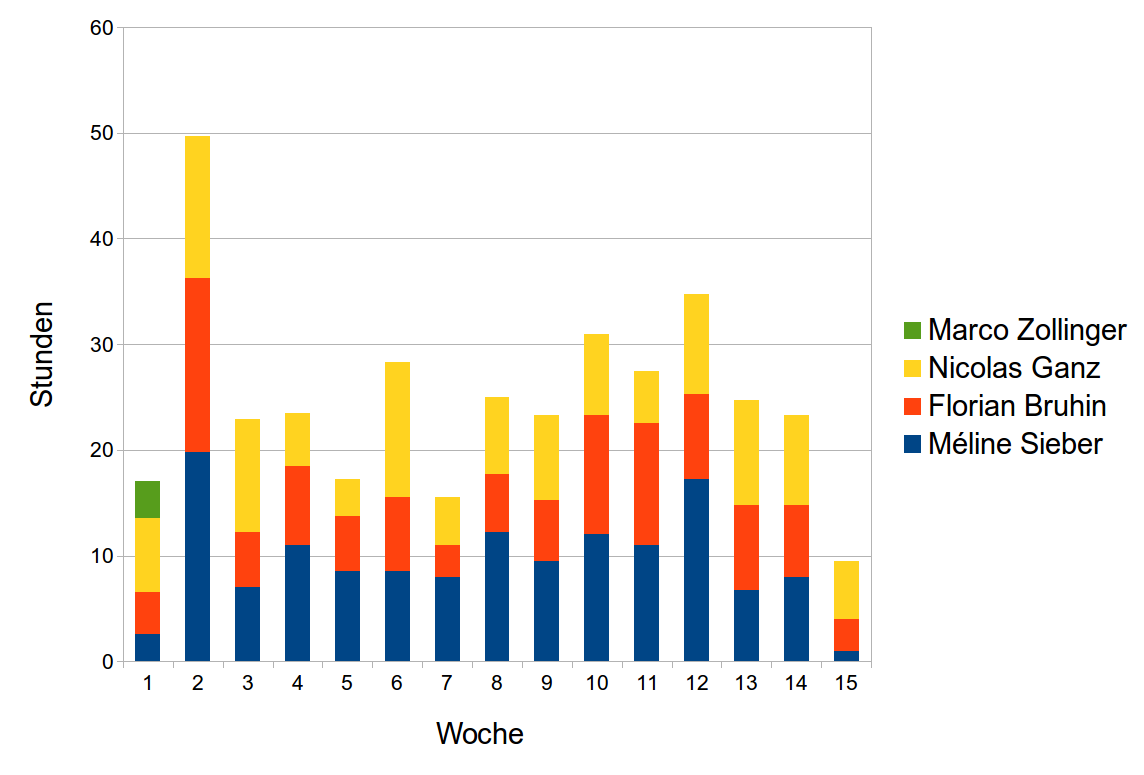
\includegraphics[width=\linewidth]{./img/time_per_person.png}
  \caption{Zeitauswertung pro Person\protect\footnotemark}
\end{figure}
\footnotetext{Stand: 31. Mai 2018, 14:23 Uhr}

In dieser Grafik sind sämtliche Zeitaufwände pro Person dargestellt.

Es zeigt, dass wir besonders für den Projektplan in der zweiten Woche sehr viel investiert haben.
Wir haben uns dabei bereits sehr viele Gedanken gemacht, wie wir das Projekt angehen und aufbauen möchten und welche Tools wir genau verwenden. Dies ist uns im Verlauf des Projekts klar zugunsten gekommen.

Zu Beginn haben wir geschätzt, dass wir durchschnittlich 8 Stunden pro Person
und Woche aufwenden.
% FIXME rephrase?
Jetzt haben wir jeweils durchschnittlich 8.2 Stunden benötigt.
Genauere Angaben sind im Dokument \verb|KitovuTimesheet.xlsx| zu finden.

\subsection{Zeitauswertung}

\begin{figure}[H]
  \includegraphics[width=\linewidth]{./img/time_per_issue.png}
  \caption{Zeitauswertung pro JIRA-Issue\protect\footnotemark}
\end{figure}
\footnotetext{Stand: 31. Mai 2018, 14:23 Uhr}

In dieser Auswertung werden die Zeitschätzungen mit den effektiven Zeiten verglichen.
Wenn die Abweichung 0\% ist, sind die Zeitschätzungen und die effektiven Zeiten gleich.
Bei einer positiven Abweichung haben wir weniger Zeit benötigt als geschätzt;
bei einer negativen Abweichung haben wir mehr Zeit benötigt.

Eine grosse Diskrepanz zeigt sich beim \verb|FileCache|.
Dabei haben wir mit Pair-Programming, Besprechungen und genauem Analysieren von Edge-Cases mehr Zeit benötigt als erwartet.

\subsection{Risikoauswertung}

Im Projektplan wurden verschiedene Risiken des Projekts
identifiziert\footnote{Projektplan, 5.2 ``Risiken''} welche zum Zeitpunkt der
\emph{End of elaboration} schon genauer untersucht wurden\footnote{End of
Elaboration / Software-Architektur-Dokument, 4. ``Architektonische Ziele und
Einschränkungen''}. Hier soll nochmals eine abschliessende Beurteilung der
Risiken vorgenommen werden.

Schon beim \emph{End of Elaboration}-Meilenstein zeigte sich, dass die
Einbindung des Studentenportals\footnote{\url{https://www.studentenportal.ch/}}
nicht funktionieren wird. Durch unsere Anfrage haben wir jedoch eine grössere
Diskussion zur Zukunft des Studentenportals
losgetreten\footnote{\url{https://github.com/studentenportal/web/issues/206}; \\
\url{https://github.com/studentenportal/web/issues/207}}. Wir sind erfreut, dass
dadurch eine Organisation für einen gemeinsamen Code-Sprint in die Gänge
geleitet wurde -- dadurch sollte das Studentenportal hoffentlich in nicht allzu
ferner Zukunft wieder wartbarer werden, als es momentan ist. Sobald dies der
Fall ist, steht nichts mehr im Wege, Support für Dokumente aus dem
Studentenportal zu \emph{kitovu} hinzuzufügen.

Ebenfalls zeigte sich durch einen ersten Prototyp, dass eine Integration von
Moodle machbar wird. Es traten einige kleinere Probleme mit der Moodle-API auf,
aber die Integration von Moodle in \emph{kitovu} funktioniert grundsätzlich. Es
fehlte uns die Zeit, um den Login-Prozess noch vollständig zu implementieren,
jedoch haben wir einen einfachen Workaround gefunden, bei dem die Nutzerin sich
via Browser einloggt und ein Authentifizierungs-Token aus den Einstellungen kopiert.

Als weitere Punkte hatten wir einen Ausfall verschiedener Infrastruktur
aufgelistet (CI/GitHub/JIRA), da diese Infrastruktur für unseren Workflow
zentral war und einige verschiedene Anbieter umspannt. Es sind keine solchen
Ausfälle aufgetreten -- jedoch fiel der Messenger-Dienst \emph{Telegram} für
unseren Chat teilweise für kurze Zeit aus. Dies stellte aber kein grösseres
Problem dar.

Schliesslich haben wir Probleme mit den verwendenten Bibliotheken und Tools
als Risiko identifiziert -- hier trat tatsächlich ein Problem auf. Das Tool
\emph{coala} welches Probleme von Code-Style-Checkern direkt in
Pull-Requests auf der richtigen Zeile kommentiert liess sich nicht korrekt
installieren. Wir haben dieses Problem
gemeldet\footnote{\url{https://github.com/coala/coala-bears/issues/2336}}, eine
Lösung steht aber weiterhin aus. Da dieses Tool nicht essentiell für unseren
Workflow war, konnten wir gut darauf verzichten.

\subsection{Code-Statistiken}

\subsubsection{Zeilen}

Laut der EPJ-Kurzanleitung sind typische Werte 4'000 Codezeilen (Netto Codezeilen, ohne Leerzeilen, ohne Kommentarzeilen). \emph{Kitovu} hat zum Zeitpunkt des Feature Freeze (16.5.2018) folgende Statistik:

\begin{tabulary}{\linewidth}{lll}
  \toprule
  \textbf{Code} & \textbf{Netto} & \textbf{Brutto} \\
  \midrule
  \emph{kitovu}-Code & 1'177 & 1'851 \\
  Test-Code & 1'405 & 2'049 \\
  \midrule
  Total & 2'582 & 3'900 \\
  \bottomrule
\end{tabulary}

Die Statistik stammt aus der PyCharm IDE und wurde mittels des ``Statistics''-Plugins erhoben.

Unser Projekt ist mit 2'582 netto Codezeilen um einiges kleiner als das typische EPJ-Projekt, andererseits haben wir auch eine Person weniger als der Durchschnitt (drei statt vier Team-Mitglieder).

\subsubsection{GitHub-Aktivität}

Auf GitHub konnte die folgende Aktivität verzeichnet werden:

\begin{tabulary}{\linewidth}{lll}
  \toprule
  \textbf{Repository} & \textbf{Commits} & \textbf{Pull-Requests} \\
  \midrule
  kitovu & 519 & 46 \\
  kitovu-docs & 223 & -- \\
  \bottomrule
\end{tabulary}

\pagebreak

\subsubsection{Testabdeckung}

Da wir schon von Beginn an einen hohen Wert auf Tests gelegt haben, fiel es uns
leicht, eine hohe Coverage mit hochqualitativen Tests zu halten:

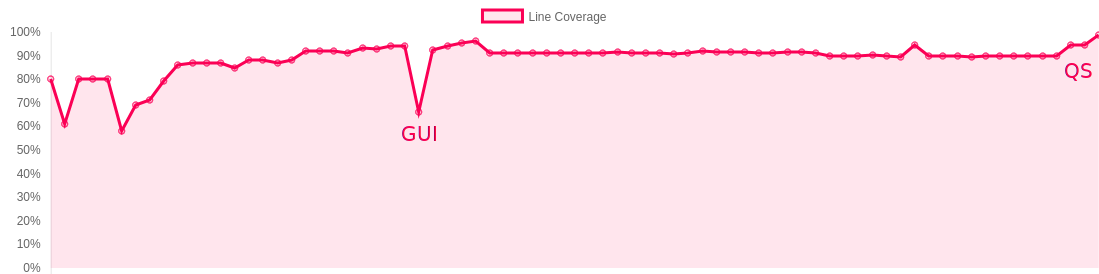
\includegraphics[width=\linewidth]{img/coverage.png}

Bei genauerer Betrachtung der Grafik fallen einige Ausreisser auf:

\begin{itemize}
  \item Wir setzten unsere Toolchain schon ganz zu Beginn des Projekts auf --
    dadurch ergaben sich am Anfang grosse Coverage-Schwankungen, da wir erstmal
    das Grundgerüst des Projekts aufgebaut haben.
  \item Die GUI wurde erst als ``proof of concept'' ohne Tests implementiert,
    diese wurden im darauffolgenden Commit aber noch nachgereicht -- die Grafik
    zeigt commits aus allen Branches, nicht nur dem \emph{master}-Branch.
  \item Zum Schluss fokussierten wir uns für das Qualitätssicherungs-Review noch
    einmal genauer auf die Tests, und ergänzten fehlende interessante Testfälle,
    was die Abdeckung nochmals verbesserte.
\end{itemize}

Wenn man die Abdeckung von einzelnen Dateien betrachtet, fällt auf, dass nur bei
der GUI/CLI kleine Teile nicht getestet sind (siehe Abbildung \ref{img:files})

\begin{figure}
  \label{img:files}
  \caption{Testabdeckung aufgeteilt auf Dateien}
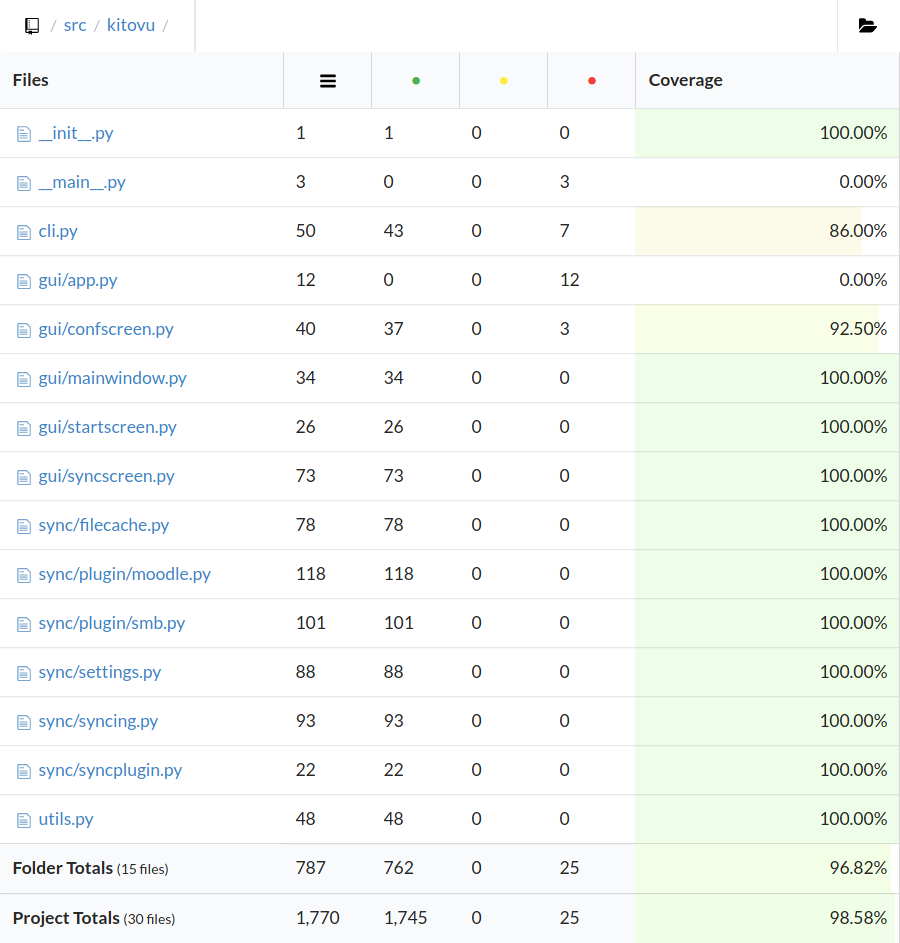
\includegraphics[width=\linewidth]{img/coverage_files.png}
\end{figure}

Unser starke Fokus auf gute Tests wurde extrem vereinfacht durch die von uns
ausgewählten Tools (pytest sowie codecov). Eine gute Testsuite war uns sehr
wichtig -- schliesslich berühren wir mit \emph{kitovu} Daten, die für Studenten
im Fehlerfall (mit persönlichen Notizen) Verluste von bis zu einem Semester
Arbeit bedeuten können. Diese Verantwortung nehmen wir ernst.

\subsection{Soll/Ist-Vergleiche}

%FIXME
 ("geschätzt/tatsächlich gemacht")


\section{Screenshots}

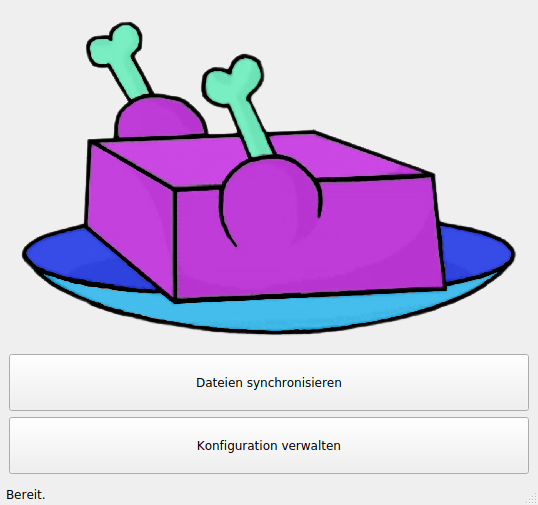
\includegraphics[width=0.5\linewidth]{./img/screenshots/gui1.png} \hspace{1em}
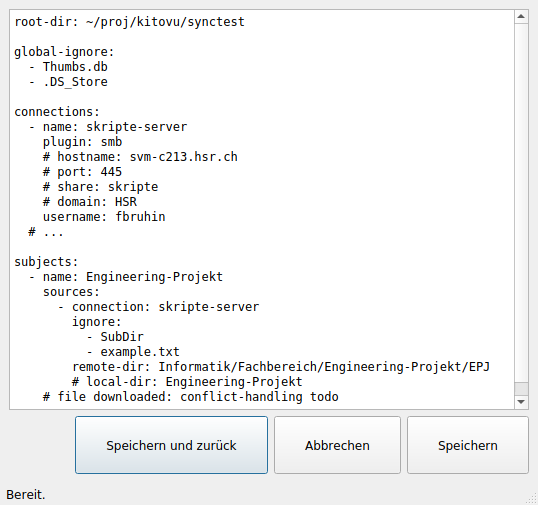
\includegraphics[width=0.5\linewidth]{./img/screenshots/gui2.png} \\[1em]
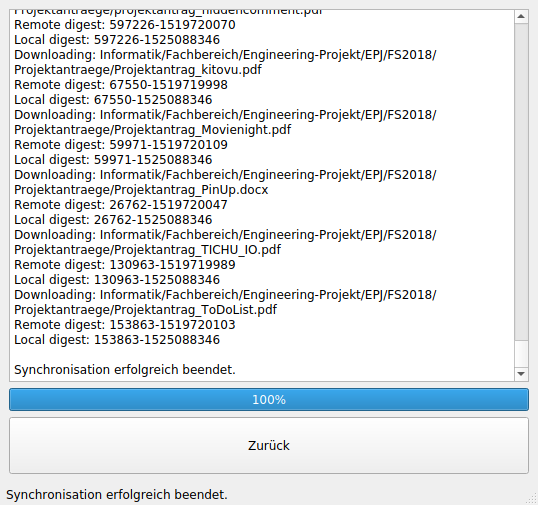
\includegraphics[width=0.5\linewidth]{./img/screenshots/gui3.png} \\
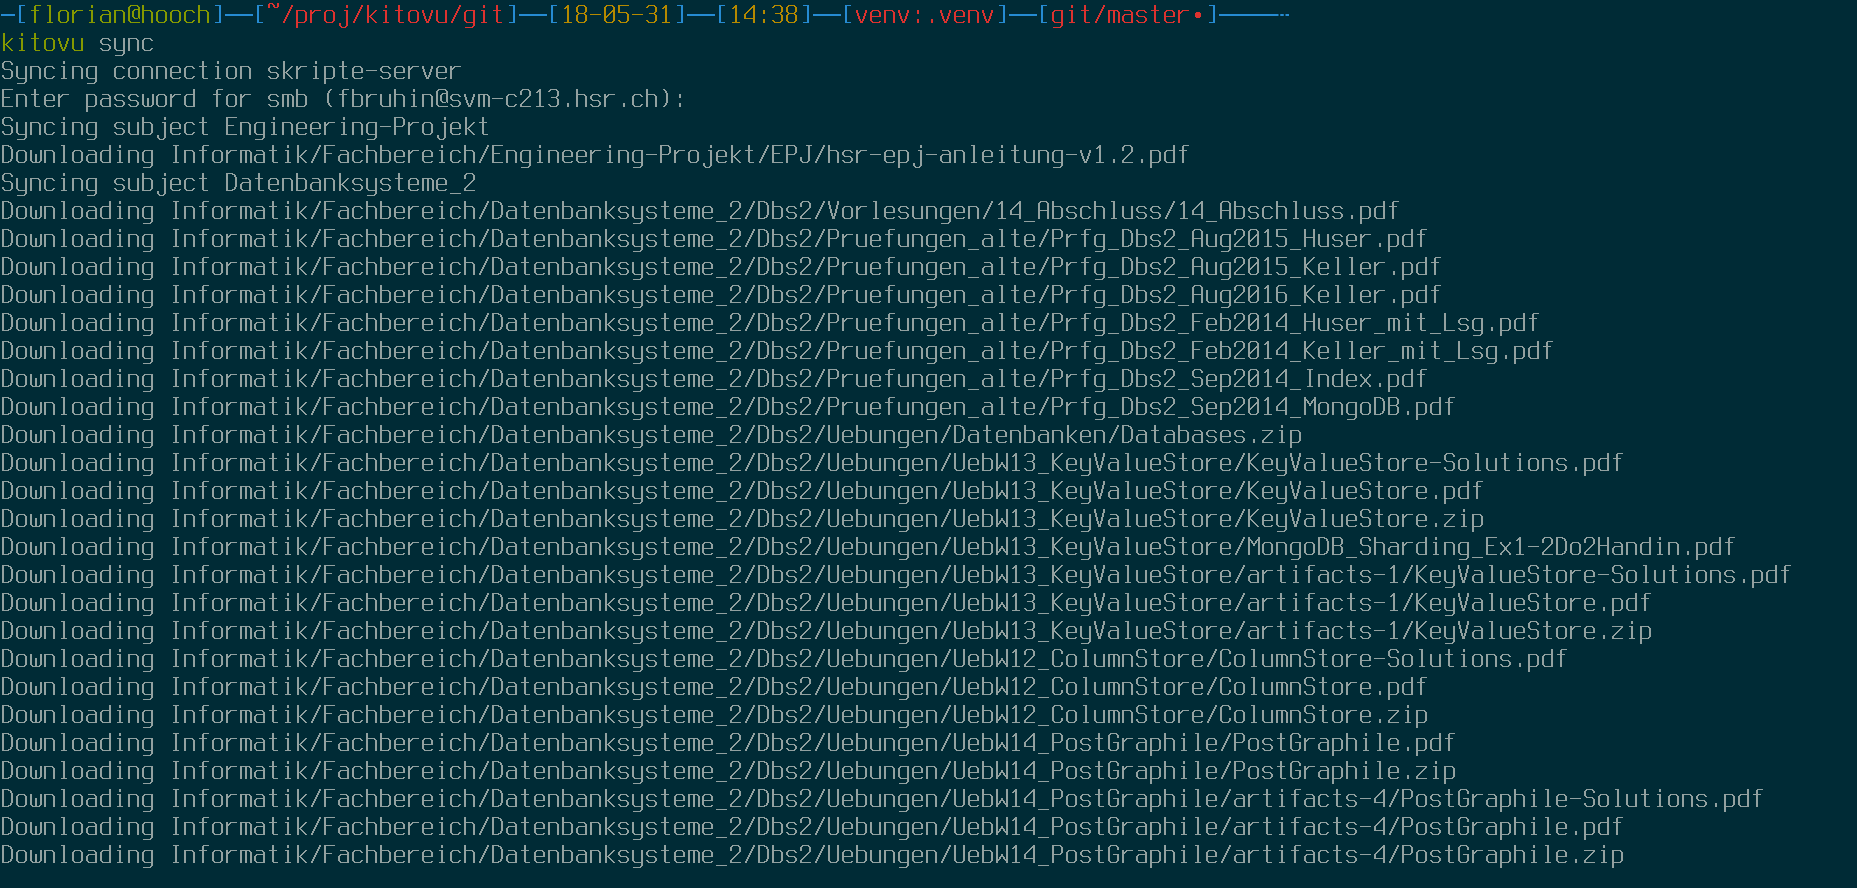
\includegraphics[width=\linewidth]{./img/screenshots/terminal.png}

\section{Installationsanleitung}

Folgende Installationsanleitung ist für die Leserinnen und Leser dieses Dokuments gedacht, die \emph{kitovu} ``in Echt'' ausprobieren möchten. Sie ist noch nicht für die effektive Verwendung gedacht, sondern für fortgeschrittene Nutzer, die das Projekt nachvollziehen möchten.

Die Installation setzt eine funktionierende, aktuelle Python-Umgebung in Version 3.6 voraus. Um diese Version parallel zu einer anderen Python-Version zu installieren, kann \emph{pyenv} verwendet werden.

Damit diese Projektversion einfach installiert und deinstalliert werden kann, erfolgt die Installation idealerweise via einer virtuellen Umgebung (\verb|virtualenv|)\footnote{Eine ausführliche Erklärung findet sich hier: \url{http://docs.python-guide.org/en/latest/dev/virtualenvs/}.}:

\begin{enumerate}
	\item Ordner mit beliebigem Namen erstellen, in dem die virtuelle Umgebung und das Projekt installiert wird, z.B. ``kitovu-test''.
	\item \verb|$ pip install virtualenv| \newline
	installiert das Python-Modul, um virtuelle Umgebungen zu erzeugen.
	\item In den Ordner ``kitovu-test'' wechseln.
	\item \verb|$ virtualenv -p /usr/bin/python3.6 kitovu| \newline
	setzt die virtuelle Umgebung auf, in einem Unterordner namens ``kitovu'', und definiert die zu verwendende Python-Version für die virtuelle Umgebung.
	\item \verb|$ source kitovu/bin/activate| \newline
	aktiviert die virtuelle Umgebung.
	\item \verb|$ pip install kitovu| \newline 
	installiert \emph{kitovu}.
	\item Eine Dokumentation zur Verwendung findet sich hier: \url{https://kitovu.readthedocs.io/}. Eine Beispielkonfiguration findet sich auf der nächsten Seite.
\end{enumerate}

Via \verb|pip install kitovu| wird \emph{kitovu} auf dem Zielrechner installiert.

Deinstallation: 

\verb|$ deactivate| deaktiviert die virtuelle Umgebung, danach kann der Ordner ``kitovu-test'' gelöscht werden.

\newpage

\subsection{Beispielkonfiguration}
	\begin{minted}[
	gobble=1,
	frame=single,
	]{yaml}
	root-dir: ~/kitovu-test/HSR
	
	global-ignore:
	  - Thumbs.db
	  - .DS_Store
	
	connections:
	  - name: skripte-server
	    plugin: smb
	    username: msieber
	  - name: moodle
	    plugin: moodle
	
	subjects:
	  - name: EPJ
	    sources:
	    - connection: skripte-server
	      remote-dir: Informatik/Fachbereich/Engineering-Projekt/EPJ
	  - name: Software Engineering 2
	    sources:
	    - connection: moodle
	      remote-dir: Software-Engineering 2 FS2018
	    - connection: skripte-server
	      remote-dir: Informatik/Fachbereich/Software-Engineering_2/SE2
	\end{minted}

\section{Projekt-Links}
\begin{tabulary}{\linewidth}{ll}
  GitHub Repository & \url{https://github.com/kitovu-bot/kitovu} \\
  GitHub Repository -- Dokumentation & \url{https://github.com/kitovu-bot/kitovu-docs} \\
  Travis CI & \url{https://travis-ci.org/kitovu-bot/kitovu/} \\
  Travis CI -- Dokumentation & \url{https://travis-ci.org/kitovu-bot/kitovu-docs/} \\
  AppVeyor CI (Windows) & \url{https://ci.appveyor.com/project/kitovu-bot/kitovu} \\
  JIRA (Issues, Projektmanagement) & \url{https://jira.keltec.ch/jira/} \\
  Confluence (Wiki) & \url{https://jira.keltec.ch/wiki/} \\
  Codecov (Coverage) & \url{https://codecov.io/gh/kitovu-bot/kitovu} \\
  Read the Docs (User-Dokumentation) & \url{https://kitovu.readthedocs.io/}
\end{tabulary}

\end{document}


